In order to keep a good structure on the program and a logical separation of functionalities, several data structures have been created.

\begin{figure}[htb]
	\centering
	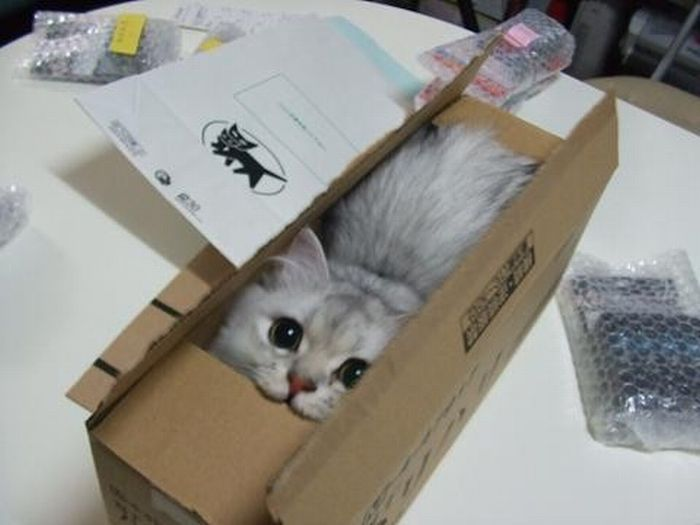
\includegraphics[width=\linewidth]{images/acatisfinetoo}
	\caption{\textit{UML diagram of the data structures.}}
	\label{fig:UML_fig} %Skapar referens till figuren
\end{figure}



\subsubsection{Frame, framelist}
DErpa derpa derpa derpa. DErpa derpa derpa derpa.DErpa derpa derpa derpa.DErpa derpa derpa derpa.DErpa derpa derpa derpa.DErpa derpa derpa derpa.DErpa derpa derpa derpa.
DErpa derpa derpa derpa.DErpa derpa derpa derpa.DErpa derpa derpa derpa.DErpa derpa derpa derpa.DErpa derpa derpa derpa.DErpa derpa derpa derpa.DErpa derpa derpa derpa.
DErpa derpa derpa derpa. As we can see in figure \ref{fig:UML_fig}. %Figurreferens

\subsubsection{Object}
DErpa derpa derpa derpa. DErpa derpa derpa derpa.DErpa derpa derpa derpa.DErpa derpa derpa derpa.DErpa derpa derpa derpa.DErpa derpa derpa derpa.DErpa derpa derpa derpa.
DErpa derpa derpa derpa.DErpa derpa derpa derpa.DErpa derpa derpa derpa.DErpa derpa derpa derpa.DErpa derpa derpa derpa.DErpa derpa derpa derpa.DErpa derpa derpa derpa.
DErpa derpa derpa derpa. See code in appendix B \ref{sec:Frame_code}.

\subsubsection{ProbabilityMap}
DErpa derpa derpa derpa. DErpa derpa derpa derpa.DErpa derpa derpa derpa.DErpa derpa derpa derpa.DErpa derpa derpa derpa.DErpa derpa derpa derpa.DErpa derpa derpa derpa.
DErpa derpa derpa derpa.DErpa derpa derpa derpa.DErpa derpa derpa derpa.DErpa derpa derpa derpa.DErpa derpa derpa derpa.DErpa derpa derpa derpa.DErpa derpa derpa derpa.
DErpa derpa derpa derpa.
